\section*{Aufgabe 5}

Es seien M, N, K beliebige Mengen.\\
Veranschaulichen Sie mit Hilfe von Venn-Diagrammen die folgenden Identitäten:\\

a) $M \ \backslash \ (N \ \backslash K) = (M \ \backslash \ N) \cup (M \cap K)$

\begin{figure}[h]
\begin{center}
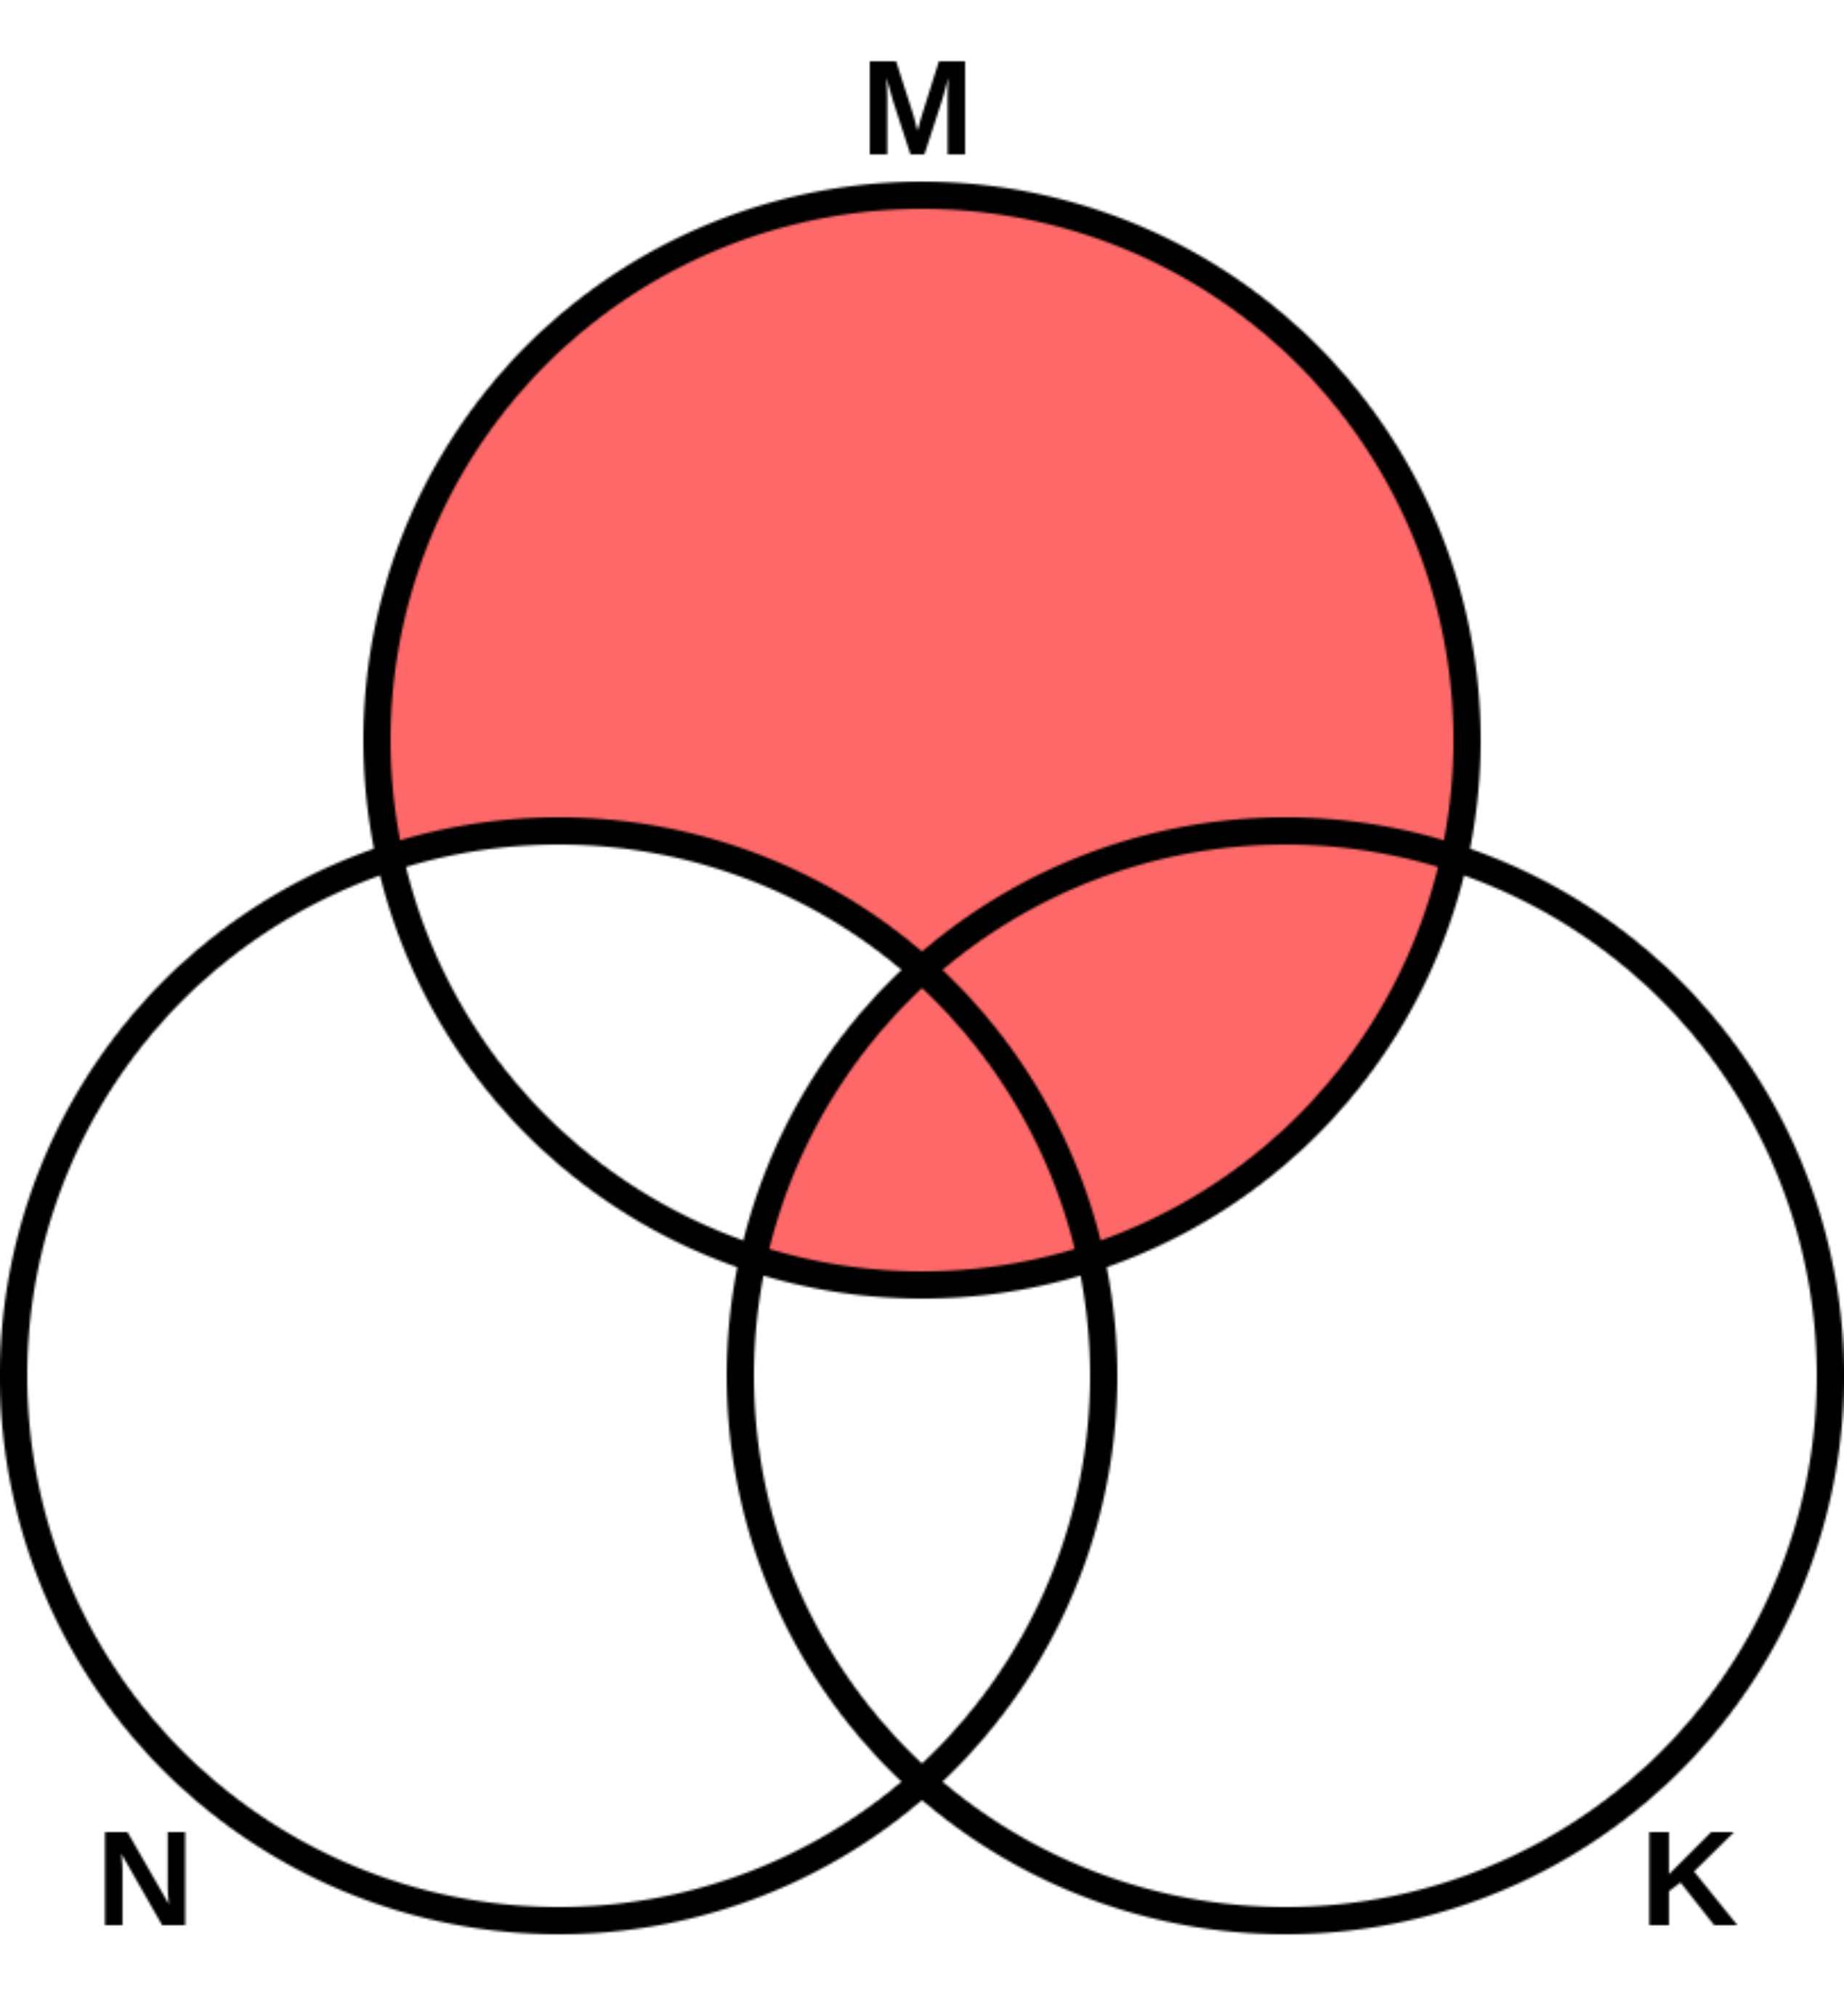
\includegraphics[width=0.3\textwidth]{graphics/venn1.png}
\caption{$M \ \backslash \ (N \ \backslash K) = (M \ \backslash \ N) \cup (M \cap K)$}
\end{center}
\end{figure}

b) $(M \ \backslash \ N) \backslash K = (M \ \backslash \ K) \backslash N$

\begin{figure}[h]
\begin{center}
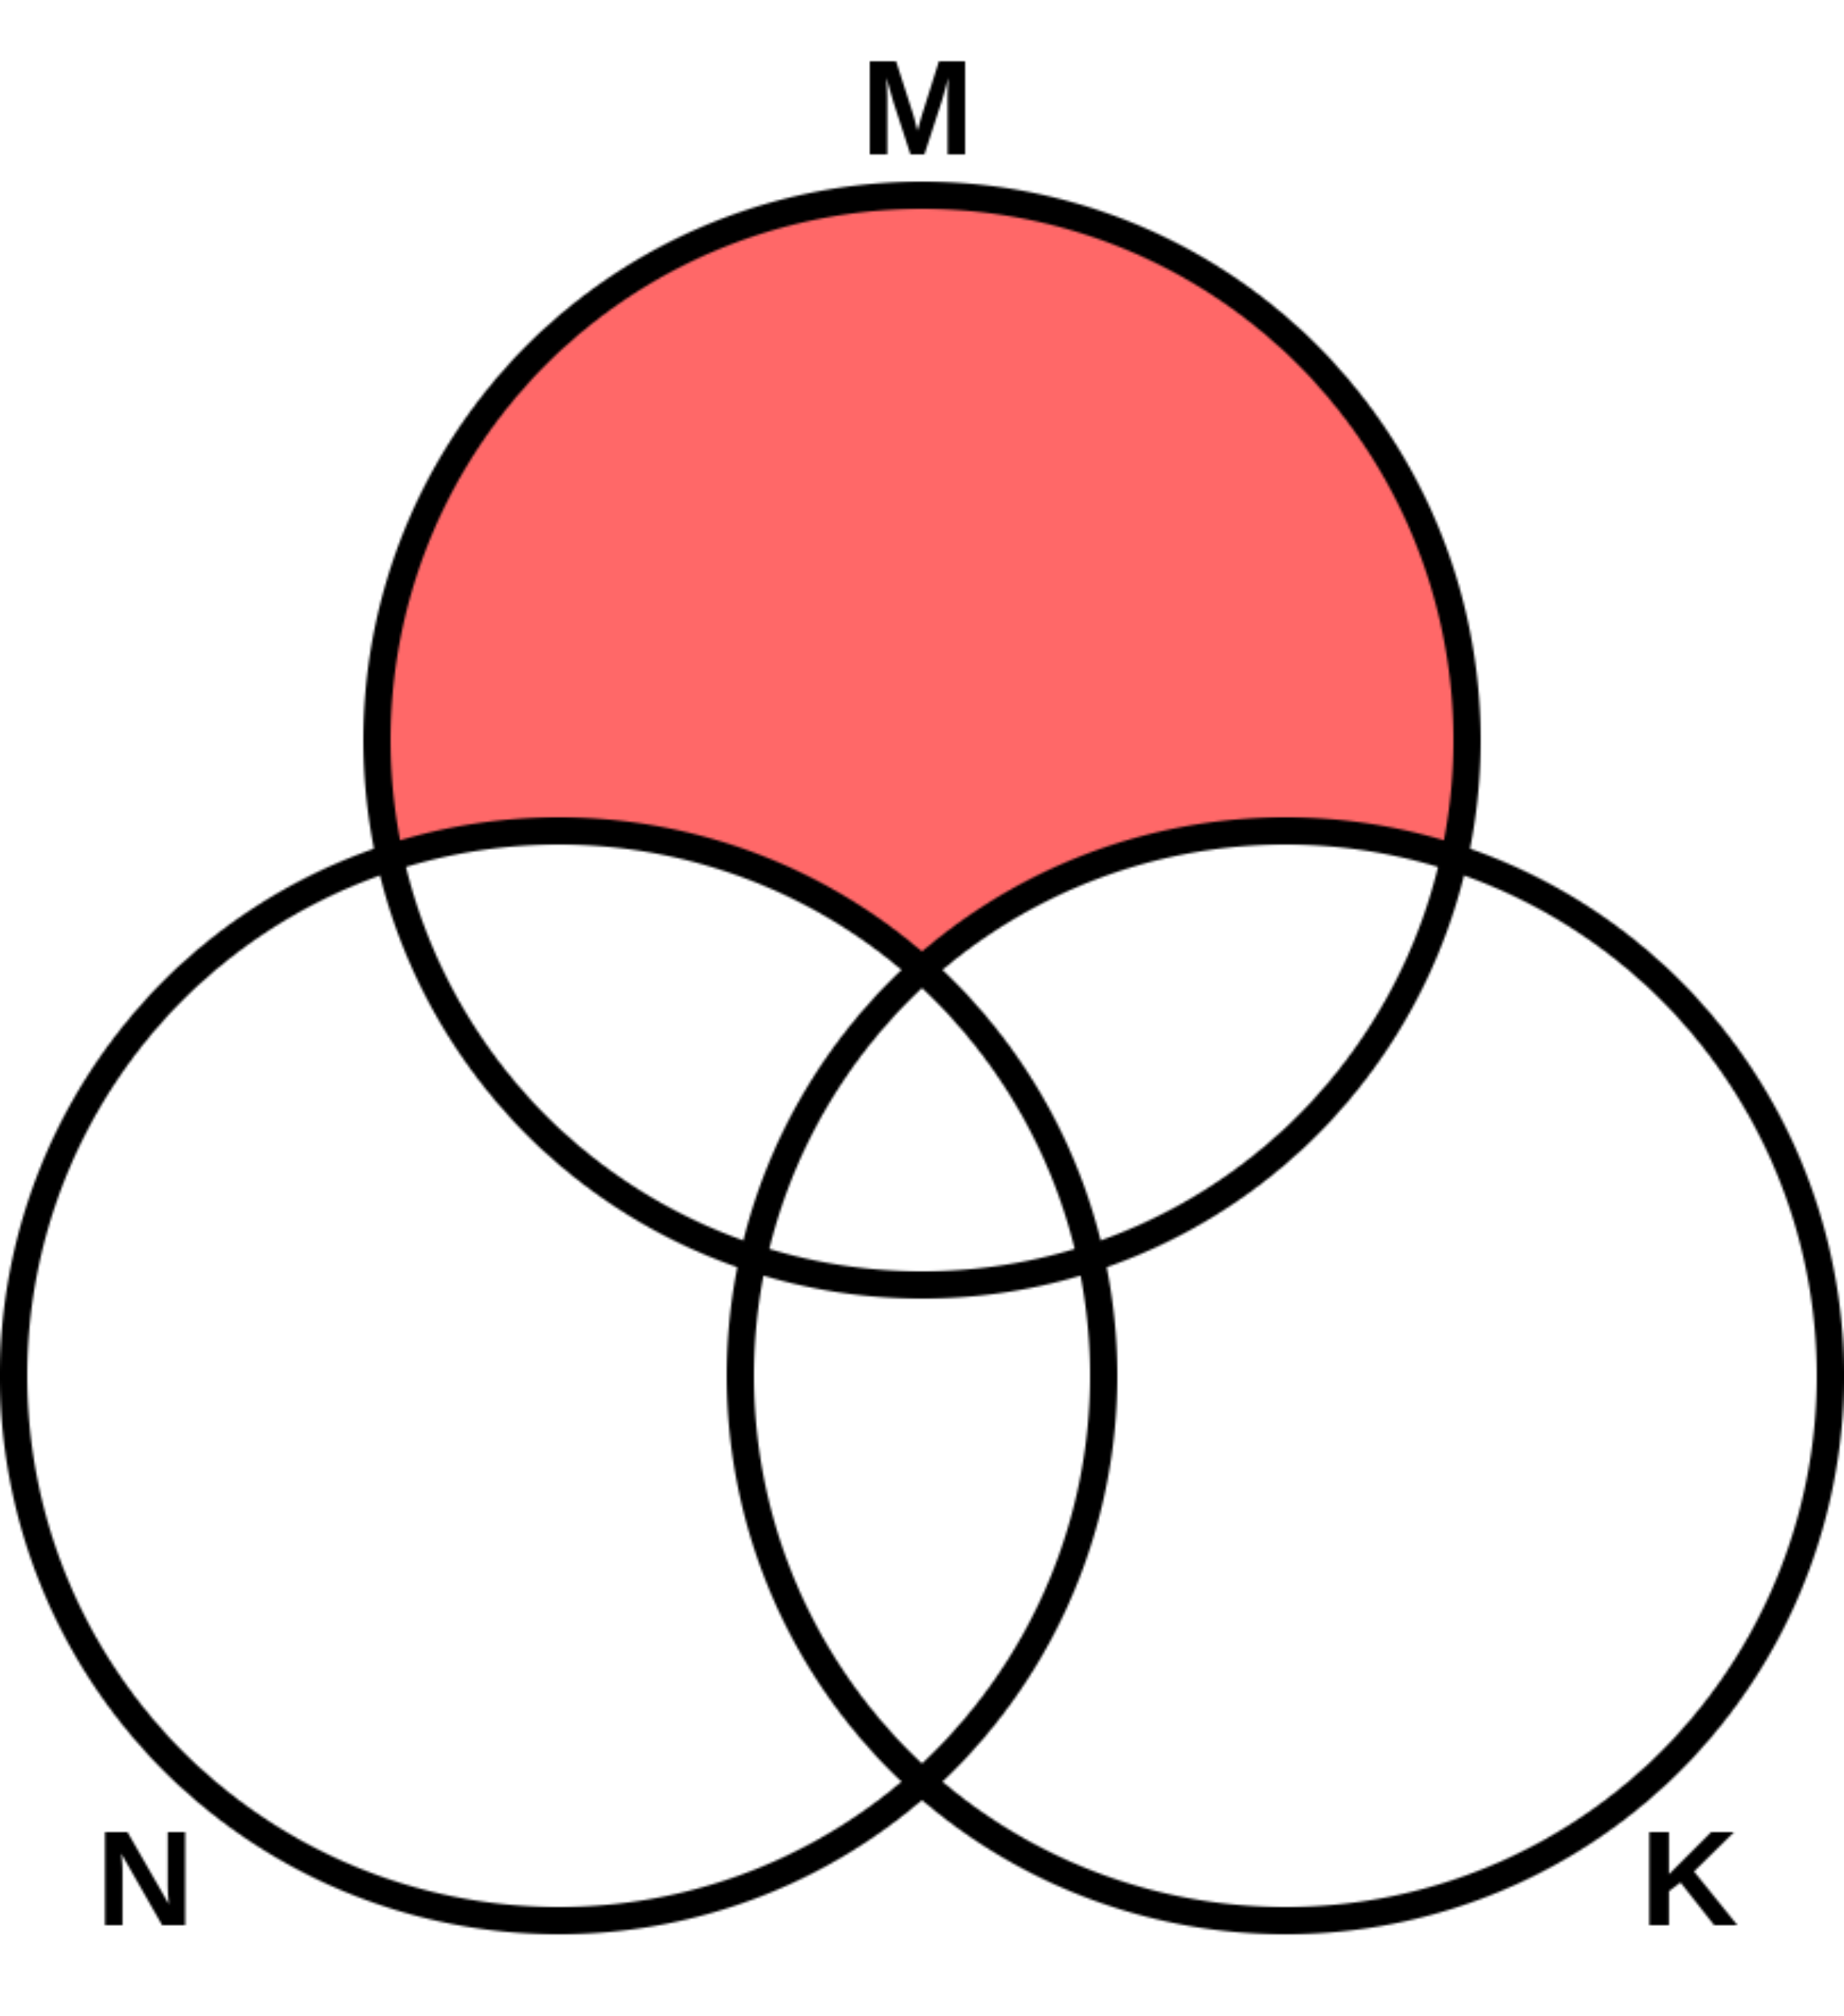
\includegraphics[width=0.3\textwidth]{graphics/venn2.png}
\caption{$(M \ \backslash \ N) \backslash K = (M \ \backslash \ K) \backslash N$}
\end{center}
\end{figure}

\newpage